\documentclass[11pt]{beamer}

\mode<article> % only for the article version
{
  \usepackage{fullpage}
  \usepackage{hyperref}
}
\usepackage{multimedia}
\usepackage{pgf,pgfarrows,pgfnodes,pgfautomata,pgfheaps,pgfshade}
\usepackage{amsmath,amssymb}
%\usepackage[latin1]{inputenc}
%\usepackage{colortbl}
\usepackage[english]{babel}
%\usepackage{fancybox}
\usepackage{hyperref}
\usepackage{graphicx}
\usepackage{ctex}
\usepackage{xeCJK}
\usepackage{fontspec,xltxtra,xunicode}
\usepackage{media9}
\usepackage{ulem}
\mode<presentation> {
  \setbeamertemplate{background canvas}[vertical shading][bottom=white!10,top=blue!10]
  
  %\usetheme{Hannover} %...The third theme
  \usetheme{Montpellier} %...The second theme
  %\usetheme[hideothersubsections]{Marburg} %....The first theme
  \usecolortheme{sidebartab}	
  \usefonttheme[onlymath]{serif}
  \setbeamercovered{invisible}
  %\pgfdeclareimage[height=1.5cm]{logo}{1111021021} \logo{\pgfuseimage{logo}}
  %\pgfdeclareimage[height=6cm]{NCKUSC}{NCKUSC} \logo{\pgfuseimage{NCKUSC}}
}

%\setbeamercolor{math text}{fg=green!50!black}
%\setbeamercolor{normal text in math text}{parent=math text}


\usepackage{lmodern}
%\usepackage[T1]{fontenc}

\usepackage{times}

\setbeamercovered{dynamic}


%\useoutertheme{split}
%\useinnertheme[shadow]{rounded}
\title{Soap Film \& Minimal Surface}
\subtitle{應用數學方法期末報告}
\author{蔡忠廷、傅鈺融、李昱勳}

\institute{Dept. of Math, NCKU, Tainan}
\date{\today}
%\nodate

\begin{document}
\noindent
\frame{\titlepage}
\begin{frame}
  \frametitle{Outline}
  \tableofcontents
  % You might wish to add the option [pausesections]
\end{frame}

\section{計劃目的}

\begin{frame}{計劃目的}
\begin{itemize}
\item 動機:
\begin{center}
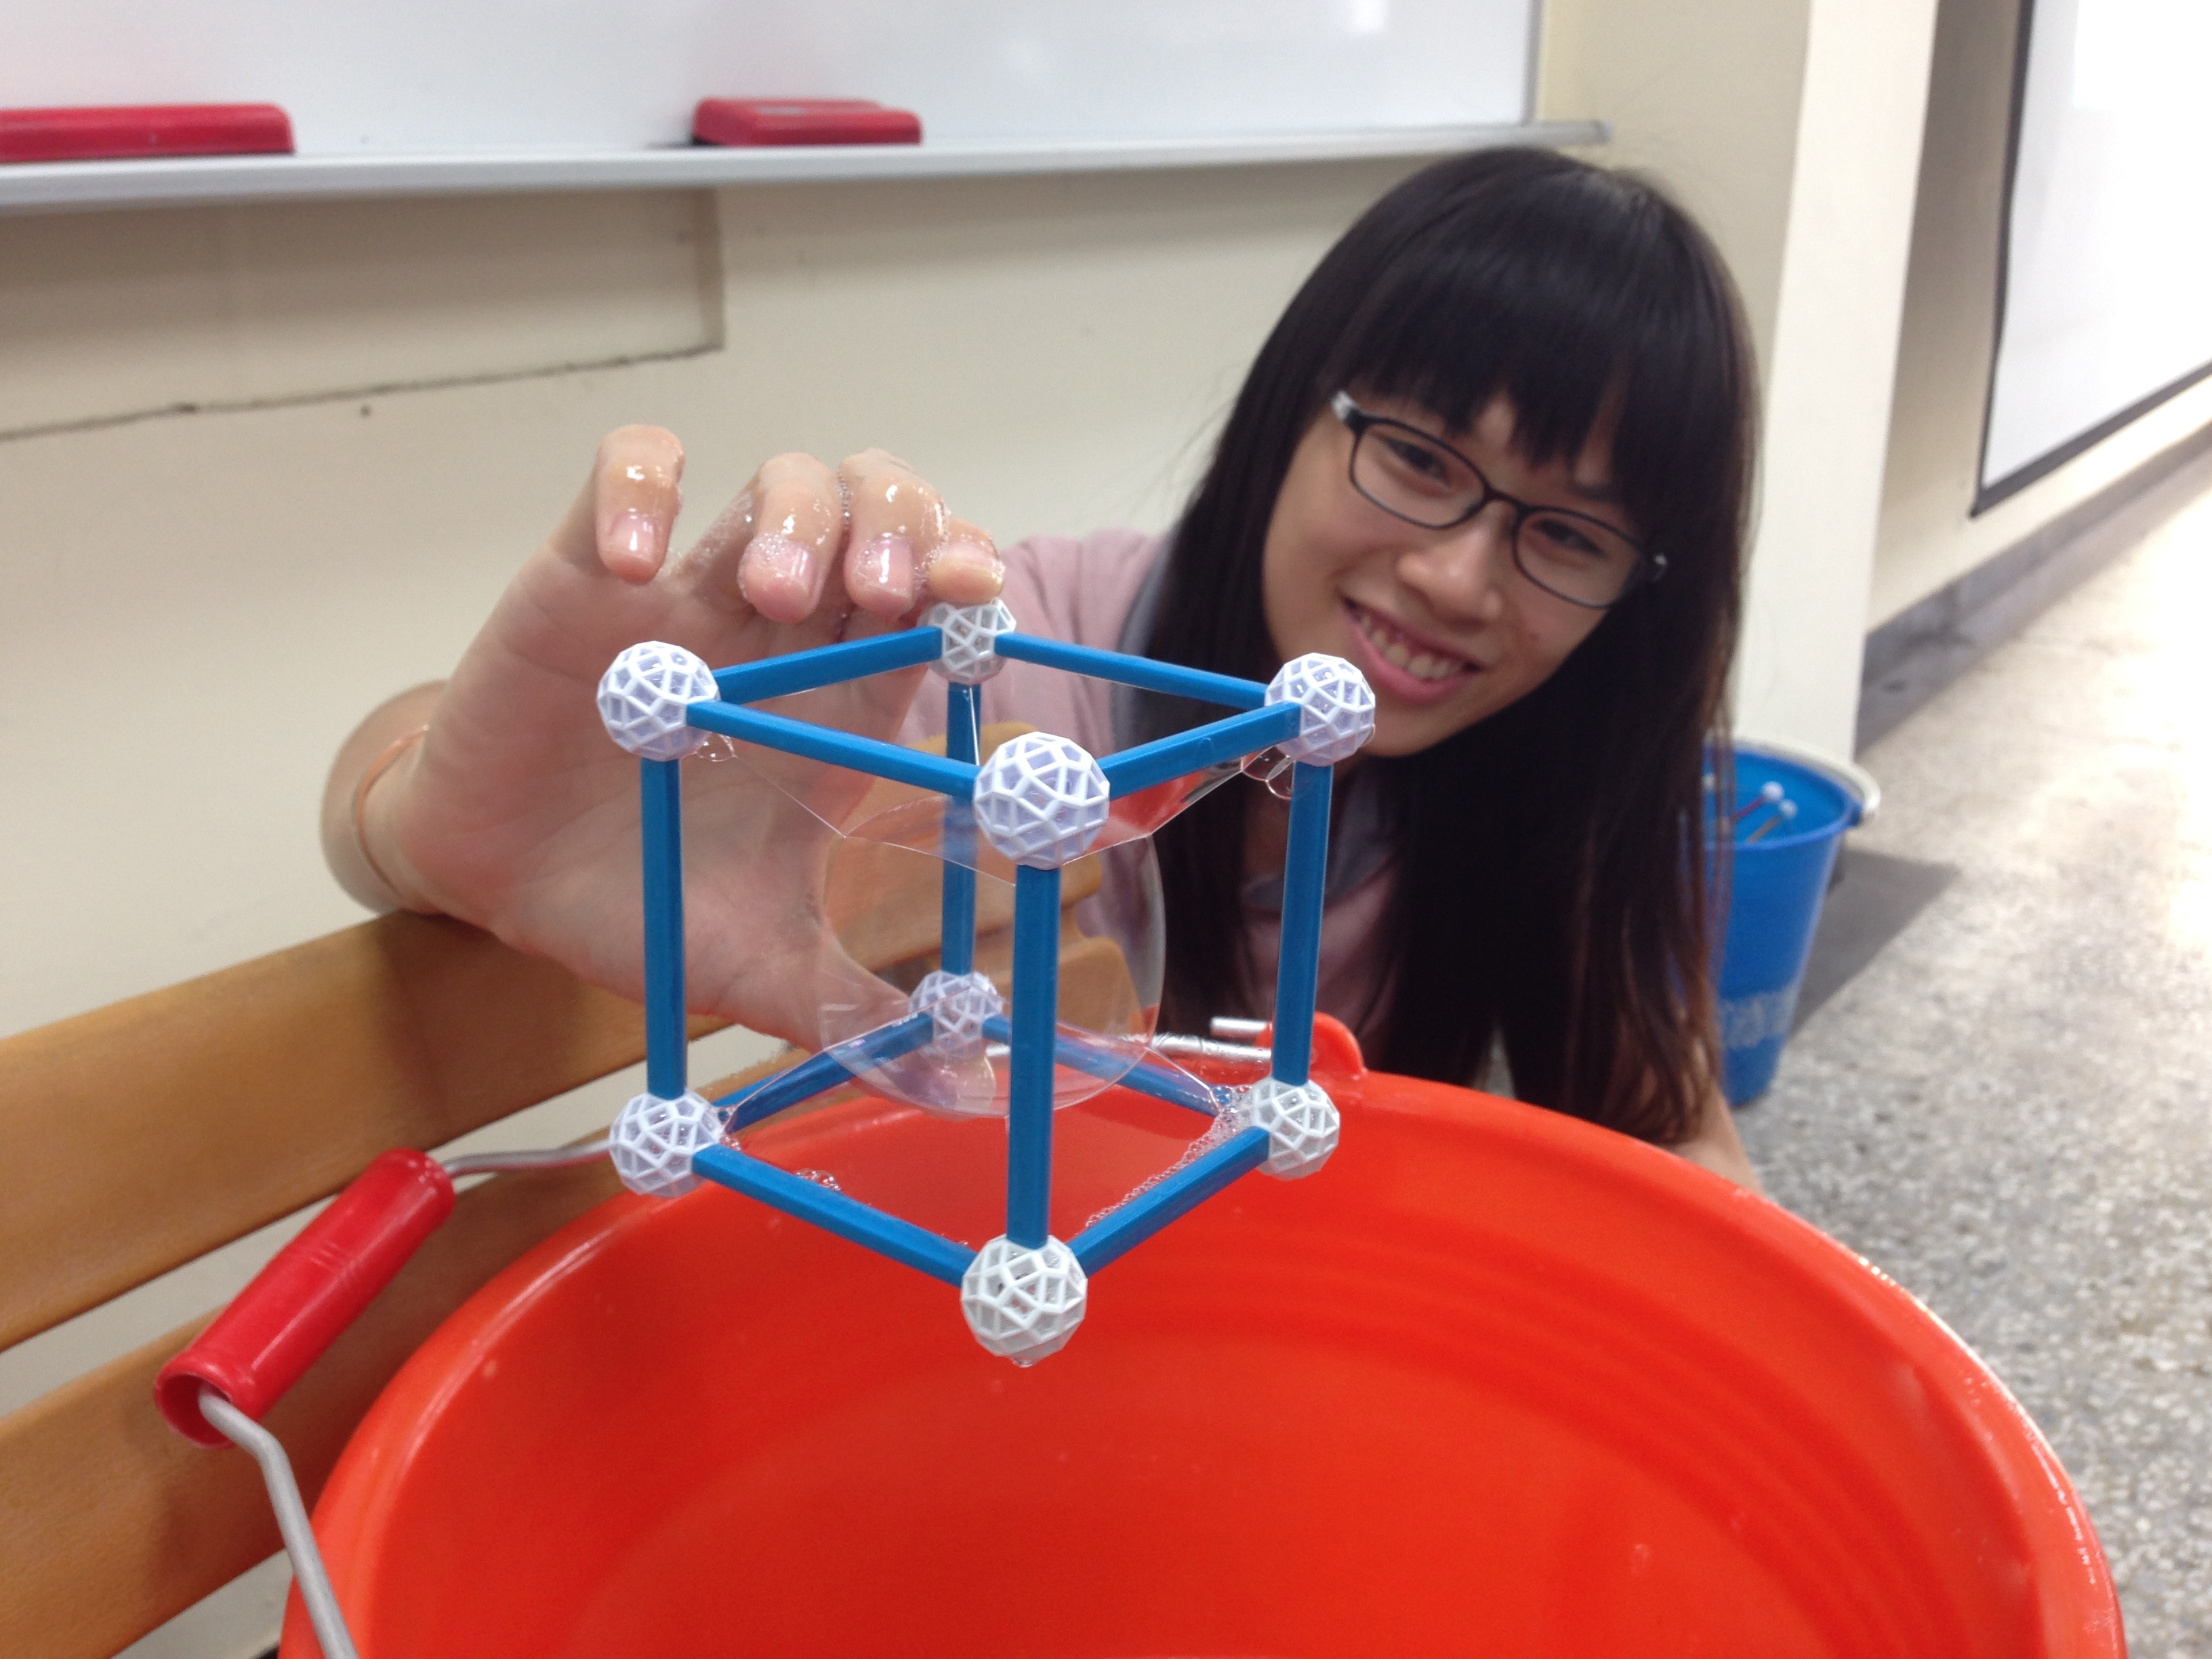
\includegraphics[width=7.5cm]{IMG_3854}
\end{center}

\end{itemize}

\end{frame}
\begin{frame}{計劃目的}
\begin{itemize}
\item 計劃目的:
使用 MATLAB 模擬出生活中的最小曲面。

\end{itemize}
\end{frame}
\section{計劃內容}
\begin{frame}{Problem}
給定框架(肥皂泡吹製器)\\肥皂泡膜形成的(曲)面有最小表面積\\[0.5cm]
\begin{tabular}{ll}
Method & Discussion\\
\pause 從最小能量下手 & \pause 理論推導不易?\\

\pause 從方程式下手&  \pause 知道的事實不多\\

\pause 從圖像下手 &   \pause 以程式實驗,模擬框架從肥皂水取出後的面

\end{tabular}

\end{frame}
\begin{frame}{Problem}
經過一番\sout{(寒徹骨)}波折後決定降低維度(\ !?)\\[0.5cm]
\pause
\invisible<1>{給定一些頂點,決定連結這些點的最小路徑\\ $\Rightarrow$ Steiner Tree Problem}
\end{frame}
\begin{frame}{Steiner Tree Problem}
Steiner tree problem是一個組合最佳化問題,與最小生成樹相似,是最短網路的一種。最小生成樹(minimum spanning tree, MST)是在給定的點集和邊中尋求最短網路使所有點聯通。而最小 Steiner tree 允許在給定的點外增加額外的點,使生成的最短網路開銷最小。\end{frame}
\section{研究方法}
\begin{frame}{Method}
使用MATLAB實驗
\end{frame}

\section{結果與討論}
\begin{frame}{Results}
\begin{figure}[h]
\centering

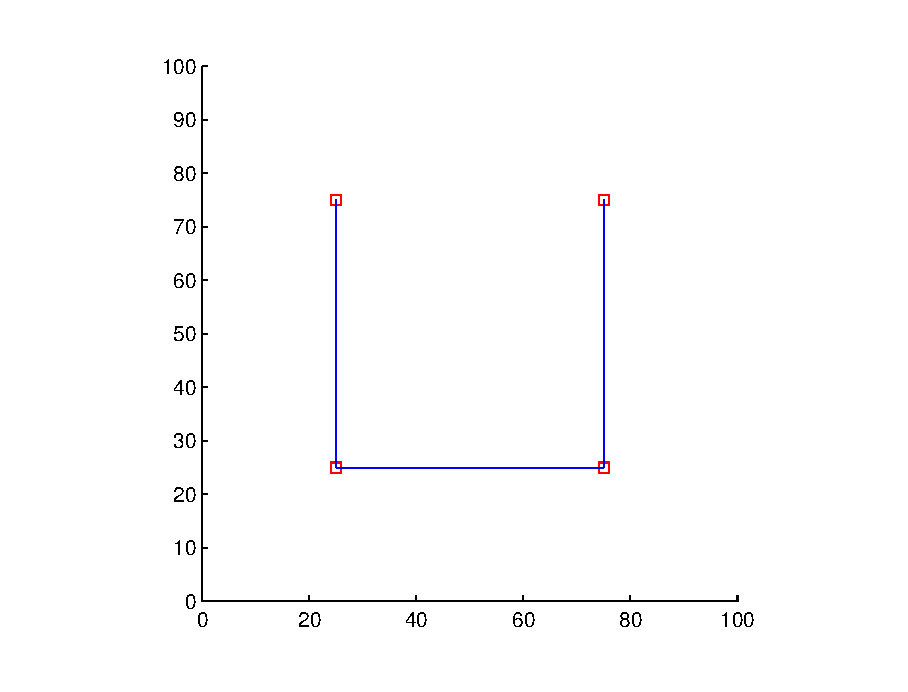
\includegraphics[width=5cm]{square1}\hfill
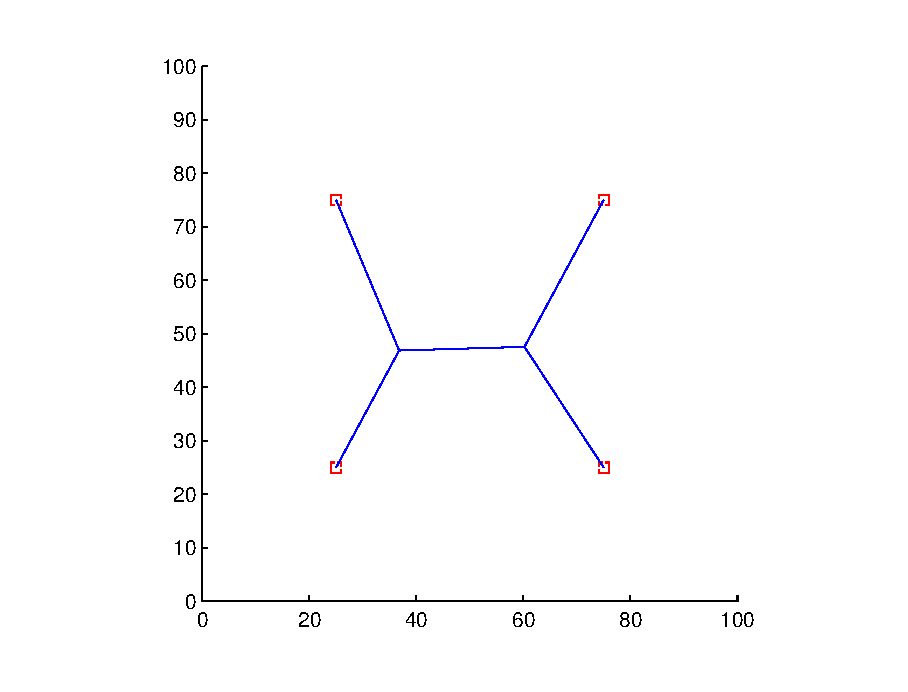
\includegraphics[width=5cm]{square2}
\caption{方形模擬結果}
\end{figure}
\end{frame}

\section{結論}
\begin{frame}{Conclusions}
三維的問題仍比二維複雜許多.......\\
\quad \quad {\tiny \sout{要最小曲面還是去吹泡泡吧}}
\end{frame}

\section{參考資料}
\begin{frame}{參考資料}
\begin{itemize}
\item Steiner Tree Problem : https://en.wikipedia.org/wiki/Steiner\_tree\_problem
\item Steiner Tree Solver : \\ http://hostel.ufabc.edu.br/$\sim$marcelo.nascimento/software.html
\end{itemize}

\end{frame}
\end{document}
